\subsection{B\'usqueda Local}

Una heur\'istica de b\'usqueda local toma una soluci\'on inicial $s$, obtenida por ejemplo a partir de una heur\'istica constructiva. Luego, en cada iteraci\'on la mejora reemplaz\'andola por otra soluci\'on, perteneciente al conjunto de soluciones vecinas de $s$. El procedimiento se repite hasta alcanzar un \'optimo local.\\
El siguiente es un esquema general de esta heur\'istica:\\
Componentes principales

\begin{itemize}
\item S = conjunto de soluciones
\item N(s) = soluciones vecinas de s
\item f(s) = valor de la soluci\'on s
\end{itemize}

Forma del algoritmo
\begin{itemize}
\item elegir una soluci\'on s $\in$ S (soluci\'on inicial)
\item mientras exista s' $\in$ N(s) donde f(s') $<$ f(s)
\begin{itemize}
	\item reemplazar s por s'
\end{itemize}
\item devolver s
\end{itemize}

\subsection{Descripci\'on del algoritmo}

Analicemos la heur\'istica de b\'usqueda local propuesta utilizando como gu\'ia el esquema general descripto en la secci\'on anterior.\\

Componentes principales
\begin{itemize}
\item S = conjunto de soluciones. En este caso, el conjunto de soluciones est\'a representado por todos los caminos entre $u$ y $v$ del grafo, que est\'en acotados por $K$ en $w_1$ y sean m\'inimos en $w_2$.
\item N(s) = soluciones vecinas de s. Dos soluciones son vecinas si comparten el camino de $w$ a $v$, donde $w$ es un nodo intermedio perteneciente al camino soluci\'on inicial. 
Es decir Sea $S=\lbrace v_1, v_2, ..., v_{x-1}, v_x \rbrace$ a soluci\'on inicial,
\\
$S' \in N(S) \Longleftrightarrow \exists v_i \in S' \diagup 
(\forall j \in \mathbb{N}, i \leqslant j < x,
\exists e \in E(S'), e=(v_j,v_{j+1}))$
\item f(s) = valor de la soluci\'on s. El valor de una soluci\'on s est\'a dado por su valor en $w_1$ y su valor en $w_2$.
\end{itemize}

Como soluci\'on inicial usamos el camino m\'inimo en $w_1$ entre $u$ y $v$, generado utilizando el algoritmo de Floyd.\\
En un principio consideramos usar tanto el camino m\'inimo en $w_1$ como el de $w_2$, pero finalmente nos decidimos por el de $w_1$ ya que, por como definimos la vecindad de una soluci\'on, si tom\'aramos el m\'inimo en $w_2$, ser\'ia probable que no est\'e acotado por $K$ y, peor a\'un, todos sus vecinos podr\'ian estar muy por arriba de esa cota. As\'i, el algoritmo hallar\'ia una soluci\'on no factible, ya que no estar\'ia acotada por $K$ y, por lo tanto, no ser\'ia ni la m\'inima ni una cercana a la m\'inima de las acotadas por ese n\'umero.\\
En cambio, tomando como base la m\'as chica en $w_1$ y suponiendo que la misma est\'a acotada por $K$ (en otro caso no existe soluci\'on para el problema); aunque al final el algoritmo no nos diera la soluci\'on exacta, tendr\'iamos al menos una buena aproximaci\'on, que seguro va a estar acotada por $K$ y que es la m\'inima entre sus vecinos (local) en $w_2$.\\
Una vez que tenemos la soluci\'on inicial $s$ entramos en el ciclo que se encarga de mejorarla utilizando sus vecinas.\\
Como definimos m\'as arriba, dos soluciones son vecinas si difieren en el camino de $u$ a $w$ (donde $w$ es un nodo intermedio del camino) y comparten el camino de $w$ a $v$. Entonces, en nuestro algoritmo vamos a ir recorriendo una a una las aristas de la soluci\'on inicial $s_{inicial}$, y, reemplazando cada una por el camino m\'inimo en $w_2$ (que ya obtuvimos al correr Floyd) entre los extremos de la misma, siempre y cuando el camino formado siga estando acotado por $K$.\\ 
As\'i, al terminar de recorrer las aristas de $s_{inicial}$ tenemos un camino acotado por $K$ que adem\'as es el m\'inimo de la vecindad de $s_{inicial}$ en $w_2$.\\
Por otro lado, inicialmente (en la primera entrega del tp), cre\'imos que ir borrando los nodos repetidos en cada iteraci\'on mejorar\'ia nuestra heur\'istica, sin darnos cuenta de que podr\'amos romper la vecindad. Por lo tanto decidimos analizar esta situaci\'on y entendemos que no es as\'i ya que, por m\'as que se eliminen nodos intermedios, mientras siga existiendo un nodo $w$ tal que de all\'i hasta $v$ el camino se preserve, seguiremos manteniendo nuestra vecindad.

\newpage
\subsection{Algoritmo}
\subsection{Algoritmo}
\lstset{language=C++,
                basicstyle=\ttfamily\footnotesize,
                keywordstyle=\color{blue}\ttfamily,
                stringstyle=\color{red}\ttfamily,
                commentstyle=\color{green}\ttfamily,
                morecomment=[l][\color{magenta}]{\#},
                breaklines=true
}
\begin{lstlisting}

void heuristicabl::execute(graph * grafo) {

	vector<vector<double> > pesos1_orig = grafo->get_weights1();
	vector<vector<double> > pesos2_orig = grafo->get_weights2();
	
	Algoritmos* algoritmo = new Algoritmos();

	vector<vector<double> > pesos1 = grafo->get_weights1();
	vector<vector<int> > floyd1 = algoritmo->floyd(pesos1);

	vector<int> camino1 = algoritmo->reconstruirPathFloyd(u,v,floyd1);
	
	if(!pesoEnRegla(camino1,pesos1_orig,k)) {
		cout << "no" << endl;
		return;
	}

	vector<vector<double> > pesos2 = grafo->get_weights2();
	vector<vector<int> > floyd2 = algoritmo->floyd(pesos2);
	
	vector<int> camino2 = algoritmo->reconstruirPathFloyd(u,v,floyd2);

	if(pesoEnRegla(camino2,pesos1_orig,k)) {
		imprimirSolucion(camino2, pesos1_orig, pesos2_orig);
		delete algoritmo;
		return;
	}
	
	for(unsigned int j=0; j<camino1.size()-1; j++) {
		vector<int> tramoCamino2 = algoritmo->reconstruirPathFloyd(camino1[j],camino1[j+1], floyd2);
		vector<int> caminoNuevo = switchTramo(camino1, tramoCamino2, j);
		borrarRepetidos(caminoNuevo);
		if(pesoEnRegla(caminoNuevo,pesos1_orig,k)) {
			camino1 = caminoNuevo;
		}
	}
	
	delete algoritmo;

	borrarRepetidos(camino1);
	imprimirSolucion(camino1, pesos1_orig, pesos2_orig);
}

vector<int> switchTramo(vector<int> camino1, vector<int> tramoNuevo, int nodoSource) {
	unsigned int sizeCamino1 = camino1.size();
	unsigned int sizeTramoNuevo = tramoNuevo.size();

	vector<int> caminoNuevo = vector<int>(sizeCamino1 + sizeTramoNuevo - 2, 0);

	for(int i=0; i<=nodoSource; i++) {
		caminoNuevo[i] = camino1[i];
	}

	for(int i=nodoSource+1; i<(nodoSource + sizeTramoNuevo - 1); i++) {
		caminoNuevo[i] = tramoNuevo[i-nodoSource];
	}

	for(unsigned int i=nodoSource+sizeTramoNuevo - 1; i<caminoNuevo.size(); i++) {
		caminoNuevo[i] = camino1[i-sizeTramoNuevo+2];
	}
	
	return caminoNuevo;
}

void borrarRepetidos(vector<int>& v) {
    int i=v.size() - 1;
    int j=i-1;
    list<int> camino;
    while(i>=0) {
        camino.push_back(v[i]);
        int aux = j;
        while(aux >= 0) {
            if(v[aux] == v[i]) {
            	j = aux-1;
            }
            aux--;
        }
        i=j;
        j--;
    }
    v = vector<int>(camino.size(), 0);
    for(unsigned int x=0; x<v.size(); x++) {
        v[x] = camino.back();
        camino.pop_back();
    }
}

\end{lstlisting}

\newpage
\subsection{Familia de grafos}
\subsubsection{Familia sin soluci\'on \'optima}
La heur\'istica de b\'usqueda local parte de una soluci\'on inicial y la va mejora de acuerdo a su vecindad. Por lo tanto, si la soluci\'on \'optima se encuentra por fuera de la vecindad no habr\'ia forma de obtenerla. Es decir, al igual que en la greedy, podemos notar que solo evaluamos una parte del grafo, y nos desentendemos del reto del mismo, por lo tanto siempre vamos a tener estos casos donde la soluci\'on \'optima va a ser inalcanzable.


\newpage
\subsection{An\'alisis de complejidad}

Al igual que en la heur\'istica greedy, aqu\'i podemos separar el anal\'isis de complidad en tres tramos:
\begin{itemize}
\item Calculo de los caminos m\'inimos con el algoritmo de Floyd que vimos que tiene complejidad O($n^3$).
\item Anal\'isis de los caso borde, el camino m\'inimo en $w_1$ y $w_2$, donde ya vimos que la complejidad es O($n$).
\item Por \'ultimo tenemos el tramo de procesamiento y generaci\'on de la soluci\'on.
Para este tramo se realizo, comentada en el c\'odigo, la evaluaci\'on de complidad, dando una cota de peor caso de 
O($n^3$) ya que son n iteraciones anidados a ciertas funciones, donde la m\'as costosa es borrarRepetidos con una 
complejidad de O($n^2$).
\end{itemize}

Como vemos en este caso tambi\'en podemos ver que, al sumar las complejidades, obtenemos una complejidad temporal de
peor caso de O($n^3$), al igual que en la heur\'istica greedy.


Veamos gr\'aficamente que efectivamente el algoritmo se comporta de la forma estimada:

\subsection{Gr\'afico de complejidad}
\begin{figure}[!hp]
	\centering
 	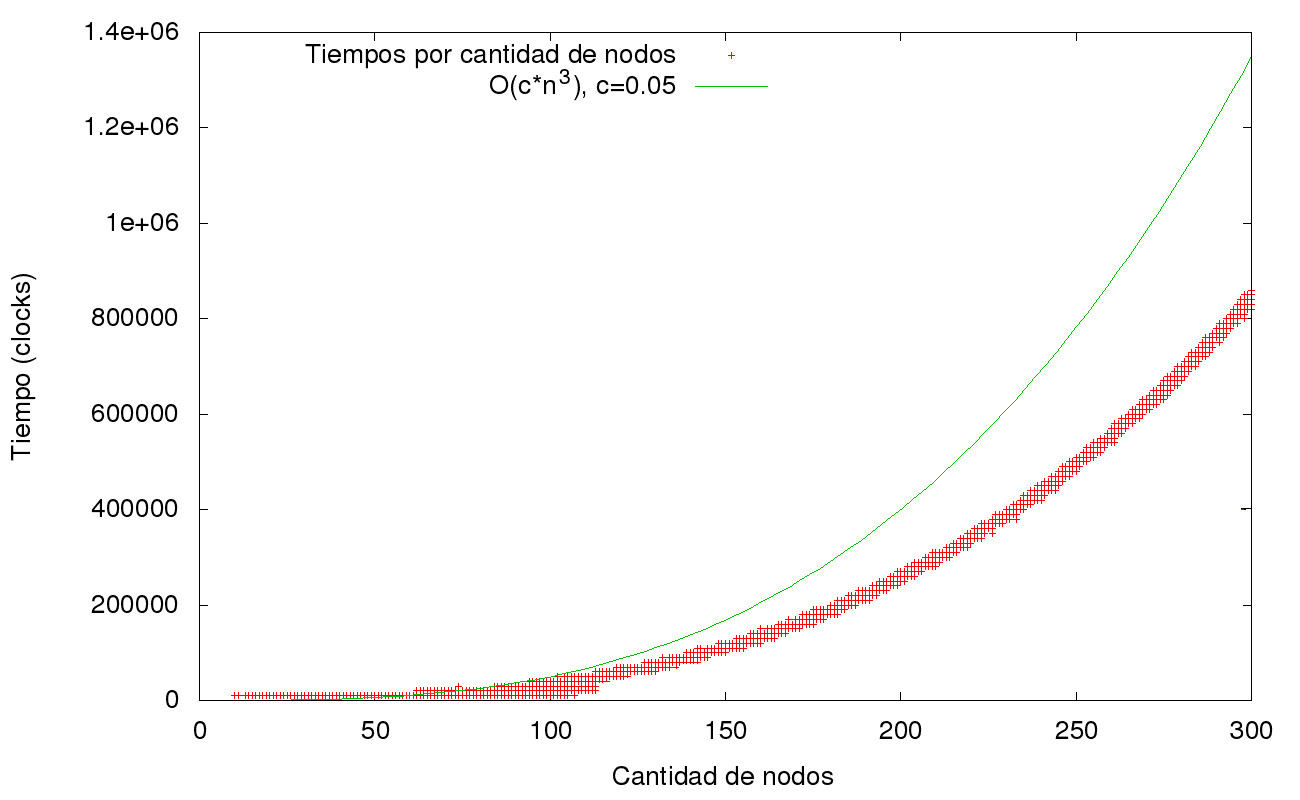
\includegraphics[scale=0.3]{img/bl_time.png}
\end{figure}


\newpage
\subsection{Experimentaci\'on}

Para la experimentaci\'on utilizamos los mismos casos de test que en la heur\'istica greedy.

Luego de las 28809 ejecuciones obtuvimos los siguientes resultados:

\subsection{Gr\'afico ejecuciones}
\begin{figure}[!hp]
	\centering
 	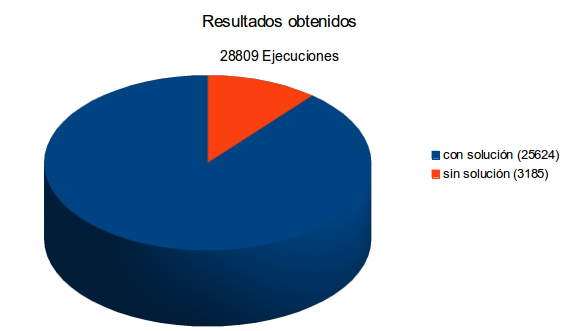
\includegraphics[scale=0.7]{img/bl_soluciones.png}
\end{figure}

En este caso tenemos 25624 casos, sobre los 28809, en los cuales hemos llegado a una soluci\'on v\'alida y 3185 en los que no se ha podido determinar un camino que cumpla con las condiciones fijadas. Es decir que en un 88,94\% hemos obtenido resultados y en el poco m\'as del 11\% restante o bien no exist\'ia soluci\'on factible o bien la heur\'istica no la ha podido hallar.

Creemos entonces que tambi\'en es necesario realizar una comparaci\'on de resultados contra el algoritmo exacto, y estos son los resultados obtenidos:

\begin{tabular}{ | l | l | l | l | l | }
\hline
ejecuciones & sin coluci\'on & con soluci\'on & iguales & distintos \\
\hline
179 & 68 & 111 & 74 & 37 \\
\hline
\end{tabular}
\\

Si recordamos los resultados de esta comparaci\'on de la heur\'istica greedy notaremos que los resultados son exactamente iguales. 
Por lo tanto decidimos de modo urgente comparar los resultados entre ambas heur\'isticas y obtuvimos que en 13 casos con resultados factibles diferentes entre ambas, dentro de las 179 ejecuciones, la heur\'istica de b\'usqueda local retornaba una soluc\'on mejor que la greedy, mientras que esta \'ultima se superpon\'ia en los 7 casos restantes.


Como conclusi\'on final y a ra\'iz de la experimentaci\'on realizada podemos ver que el comportamiento es bastante similar al presentado por la heur\'istica greedy. Y en relaci\'on con los tiempos requeridos por el algoritmo exacto, podemos decir que es completamente razonable la utilizaci\'on de estas heur\'isticas ya que tienen una complejidad temporal muchisimo menor y si le sumamos que encuentra soluciones factibles en m\'as del 80\% de los casos, en donde en un 67\% de los mismos la soluci\'on encontrada fue la misma.

